\documentclass[12pt]{article}
\usepackage[utf8]{inputenc}
\usepackage{graphicx} % Allows you to insert figures
\usepackage{amsmath} % Allows you to do equations
\usepackage{fancyhdr} % Formats the header
\usepackage{geometry} % Formats the paper size, orientation, and margins
\usepackage[style=authoryear-ibid,backend=biber]{biblatex} % Allows you to do citations - does Harvard style and compatible with Zotero
\addbibresource{Example.bib} % Tells LaTeX where the citations are coming from. This is imported from Zotero
\usepackage[english]{babel}
\usepackage{csquotes}
\usepackage{background}
\usepackage{minted}
\renewcommand*{\nameyeardelim}{\addcomma\space} % Adds comma in in-text citations
\linespread{1.5} % About 1.5 spacing in Word
\setlength{\parindent}{0pt} % No paragraph indents
\setlength{\parskip}{1em} % Paragraphs separated by one line
\renewcommand{\headrulewidth}{0pt} % Removes line in header
\geometry{a4paper, portrait, margin=1in}
\setlength{\headheight}{14.49998pt}
\backgroundsetup{scale=1,angle=0,opacity=0.175,contents={
\includegraphics[scale=0.25]{1200px-Vellore_Institute_of_Technology_seal_2017.png}}}


\begin{document}
\begin{titlepage}
\NoBgThispage
   \begin{center}
        \begin{figure}[h] % h - Place the float here, i.e., approximately at the same point it occurs in the source text (however, not exactly at the spot)
        \centering
        
\includegraphics[width=15cm]{1583124354phpJTtnK5.png}
        \end{figure}

        \Huge{Digital Assignment 1}

        \vspace{0.5cm}
        \LARGE{20BIT0380 - Hardik Nagpal\\20BIT0386 - Raghav Gupta\\20BIT0381 - Niladri Mitra\\20BIT0406 - Sanchit Sandeep Khedkar\\20BIT0015 - Atishay Jain}
       
        \vspace{2.5 cm}

        \vspace{0.25 cm}
        \Large{ITE2015 - Information Systems Audit}
        \large{VL2021220502557}
       

       \vfill
    \end{center}
\end{titlepage}
\newpage
Q. The acquaintance of system audit is very significant for all experts, as system has become an essential part of all processes. Furthermost of our work has become systemized and information technology driven so it becomes necessary for a company secretary to recognize about the basic perceptions involving to system audit.
Write a report on Information systems auditing or systems audit process, explaining what you have understood about the nature and scope of system audit; relationship between information system audit and different functions management; and the design of information system audit
plan
\par
Ans-\\
Information systems auditing is the process of attesting objectives (those of the external auditor) that focus on asset safeguarding and data integrity, and management objectives (those of the internal auditor) that include effectiveness, and efficiency both. 
The objectives are as follows-
\begin{itemize}
    \item \textbf{Data Integrity Objectives}
    \item \textbf{Objectives of system efficiency}
    \item \textbf{System Effectiveness Objectives}
    \item \textbf{Asset Safeguarding Objectives}
\end{itemize}
\newpage
Auditing an information system can be summarized by the following flowchart-
\begin{figure}[h] % h - Place the float here, i.e., approximately at the same point it occurs in the source text (however, not exactly at the spot)
\centering
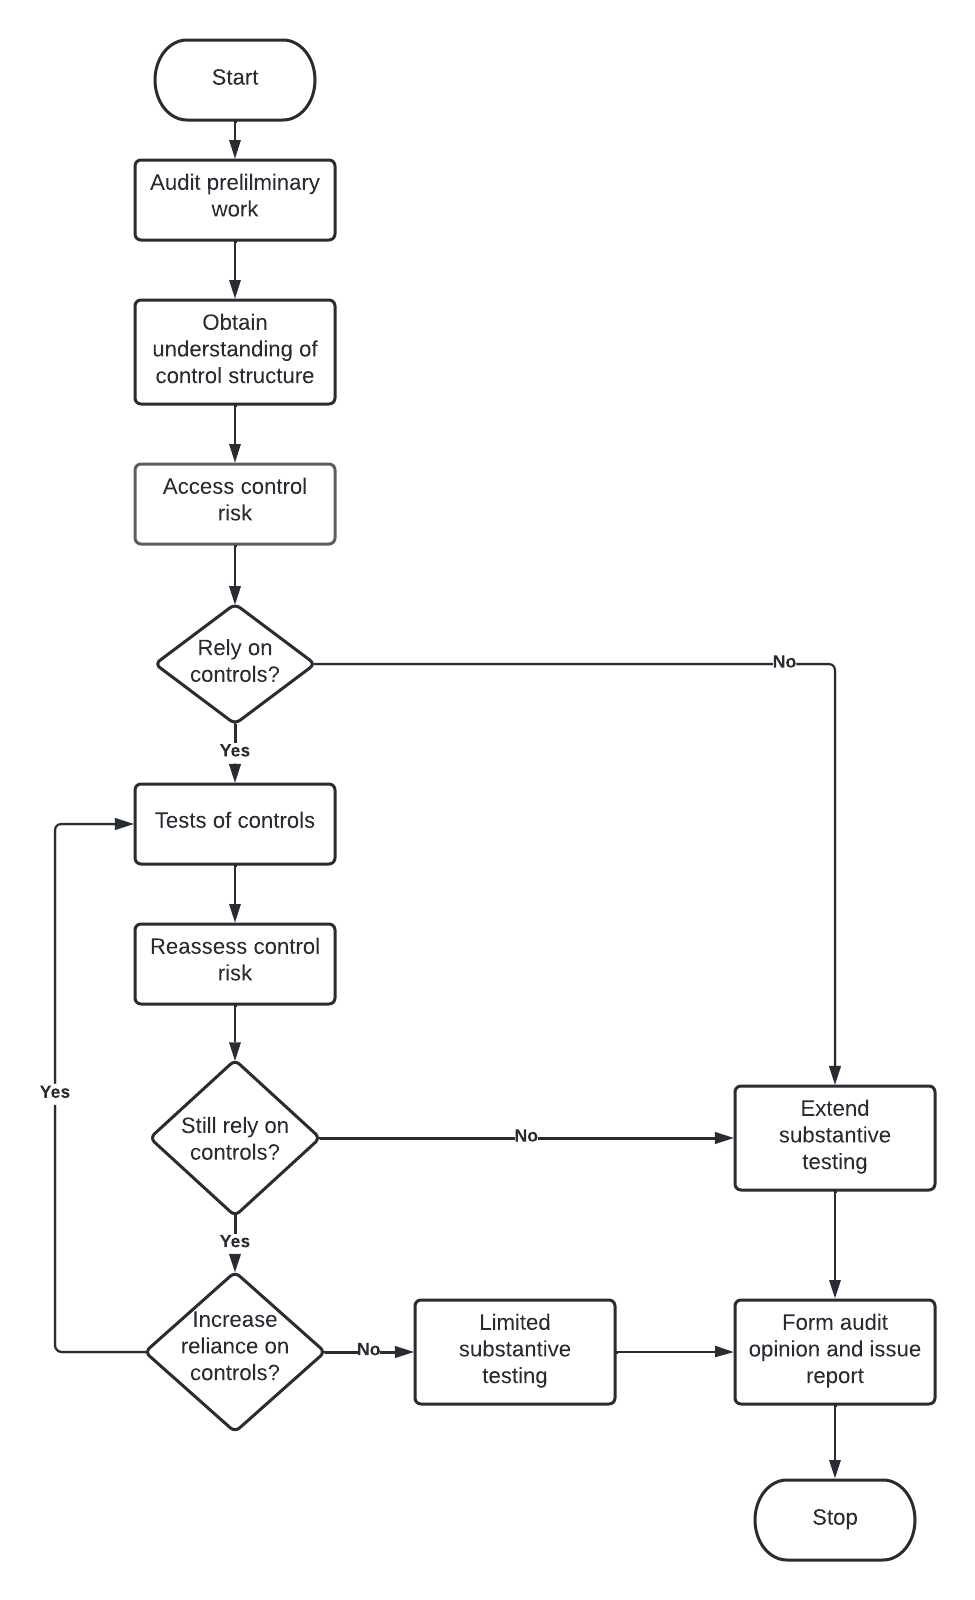
\includegraphics[scale=0.3005]{Blank diagram.png}
\end{figure}

The scope of an information system audit process should include the examination and evaluation of the adequacy and effectiveness of the system of internal controls and the quality of performance by the information system. In addition, information system audit process will also examine and evaluate the planning, organising and directing processes whether reasonable assurance exists in the objectives and goals will be achieved. The scope of the audit will also include the control system for the use and protection of information and information system such as data, applications system, technology facilities and people.
\newpage
The auditor plays a vital role in evaluating the performance of various controls under managerial controls. Some of the key areas that the auditor should pay attention while evaluating managerial controls and its types are provided below.
\par
The role of an auditor at each activity at the top managerial level is as under:
\begin{itemize}
    \item \textbf{Planning}: Evaluating whether top management has formulated a high quality information system's plan that is appropriate to the needs of an organisation.
    \item \textbf{Organising}: Concerning how well top management acquires and manages staff. This is for three reasons:
    \begin{itemize}
        \item Effectiveness of IS functions depends on quality of staff.
        \item Intense competition and high turnover have made acquiring and retaining good employees a complex activity
        \item Employees are most likely to perpetuate irregularites.
    \end{itemize}
    \item \textbf{Leading}: Examination of variables that often indicate poor leadership.
    \item \textbf{Controlling}: Focus on the subset of control activities that should be performed by top management like those aimed at ensuring that the information system function accomplishes its objectives at a global level.
\end{itemize}
Three types of audits may be conducted during the system development process:
\begin{itemize}
    \item \textbf{Concurrent Audit}: Assistance to the team in improving the quality of systems development for the specific system being built.
    \item \textbf{Post Implementation audit}: Helping an organisation learn from experiences in the development of a specific application system.
    \item \textbf{General audit}: Overall evaluation of systems development controls and determination whether the extent of substantive testing can be reduced.
\end{itemize}
\newpage
During the planning phase auditors must decide on the preliminary materiality level to be set for the audit. Auditors must also make a judgement on the desired audit risk. The level of desired risk is set for the overall audit rather than for segments of it. The levels of inherent risk will vary across different segments of the audit; some segments are more susceptible to errors, irregularities, ineffectiveness, inefficiencies. An auditor must consider each segment of the audit in turn and evaluate the factors that lead to inherent risk associated with the segment.\\ The following steps can be taken for a risk-based approach to make an audit plan:
\begin{itemize}
    \item Inventory of the systems in use and their categorisation.
    \item Determining which of the systems impact critical functions or assets, such as money, materials, customers, decision making, and how close to realtime they operate.
    \item Assessment of risks that would affect the systems and the severity of impact on the business.
    \item Decision of audit priority, resources, schedule, and frequency based on the above assessment.
\end{itemize}
\end{document}
